\chapter{Literature Survey}

This chapter begins with reviews of popular and recent web standards like WebRTC, Matrix, GraphQL and REST. 
Further sections then review existing neural network architectures, best practices, and algorithms.
Finally, the chapter ends with the review and comparison of various existing key technologies, packages
and tools.

% Tabulate the summary, pros, cons, and other stuff!

\section{WebRTC}

WebRTC (Web Real-Time Communication) is a free, open-source project providing web browsers and 
mobile applications with real-time communication via simple Application Programming Interfaces (APIs). 
It allows audio and video communication to work inside web pages by allowing direct peer-to-peer 
communication, eliminating the need to install plugins or download native apps.
It supports video, voice, and generic data to be sent between peers, allowing developers 
to build powerful voice- and video-communication solutions.~\cite{wikiWebRTC}

There are 3 primary components of the WebRTC API and each plays a unique role in WebRTC specification:

\subsubsection{MediaStream (GetUserMedia)}

The MediaStream API provides a way to access device cameras and microphones using JavaScript. 
It controls where multimedia stream data is consumed, and provides some control over the devices 
that produce the media. It also exposes information about devices able to capture and render media.

\subsubsection{RTCPeerConnection}

The Peer Connection is the core of the WebRTC standard. It provides a way for participants to 
create direct connections with their peers without the need for an intermediary 
server (beyond signalling). Each participant takes the media acquired from the media 
stream API and plugs it into the peer connection to create an audio or video feed.  
The PeerConnection API has a lot going on behind the scenes. It handles SDP negotiation, 
codec implementations, NAT Traversal, packet loss, bandwidth management, and media transfer.

\subsection{RTCDataChannel}

The RTCDataChannel API was setup to allow bi-directional data transfer of any 
type of data - media or otherwise - directly between peers. It was designed to mimic the 
WebSocket API, but rather than relying on a TCP connection which although reliable is high 
in latency and prone to bottlenecks, data channels use UDP-based streams with the configurability 
of the Stream Control Transmission Protocol (SCTP) protocol. This design allows the best 
of both worlds: reliable delivery like in TCP but with reduced congestion on the network like in UDP.

\subsection{Establishing the connection}

Before a peer-to-peer video call can begin, a connection between the two clients 
needs to be established. This is accomplished through signalling. Signalling falls 
outside of the realm of the WebRTC specification but is the vital first step in establishing 
an audio/video connection.

\subsection{Signalling}

Signalling allows two endpoints (senders, receivers, or both) to exchange metadata to 
coordinate communication in order to set up a call. This call-and-response message flow 
contains critical details about the streaming that will take place, that is, the number 
and types of streams, how the media will be encoded, etc. 

This is needed for two reasons: because the communicating peers do not know each other’s 
capabilities, and the peers do not know each other’s network addresses.

\subsection{NAT Traversal - ICE, TURN and STUN}

Once the initial signalling for a streaming connection has taken place, the two endpoints need 
to begin the process of NAT (Network Address Translation) traversal.
This assigns a public address to a computer inside a private network for setting up a real-time connection. 
In a WebRTC-enabled communication, unless the two endpoints are on the same local network, 
there will be one or more intermediary network devices (routers/gateways) between the two. 
There are three key specifications that are used in WebRTC to overcome these hurdles:

\begin{itemize}
    \item \textbf{Interactive Connectivity Establishment (ICE)} - ICE is used to find all the ways 
    for two computers to “talk to each other”. It has two main roles, gathering candidates 
    and checking connectivity. It guarantees that if there is a path for two clients to communicate, 
    it will find it and ensure it is the most efficient. It makes use of two protocols - STUN and TURN.
    \item  \textbf{Session Traversal Utilities for NAT (STUN)}  – It is a lightweight and simple 
    method for NAT Traversal. STUN allows WebRTC clients to find out their own public IP address 
    by making a request to a STUN server. 
    \item  \textbf{Traversal Using Relays around NAT (TURN) }  - The TURN server assists in the NAT 
    traversal by helping the endpoints learn about the routers on their local networks, 
    as well as blindly relaying data for one of the endpoints where a direct connection is 
    not possible due to firewall restrictions.
\end{itemize}

\begin{figure}
\begin{center}
    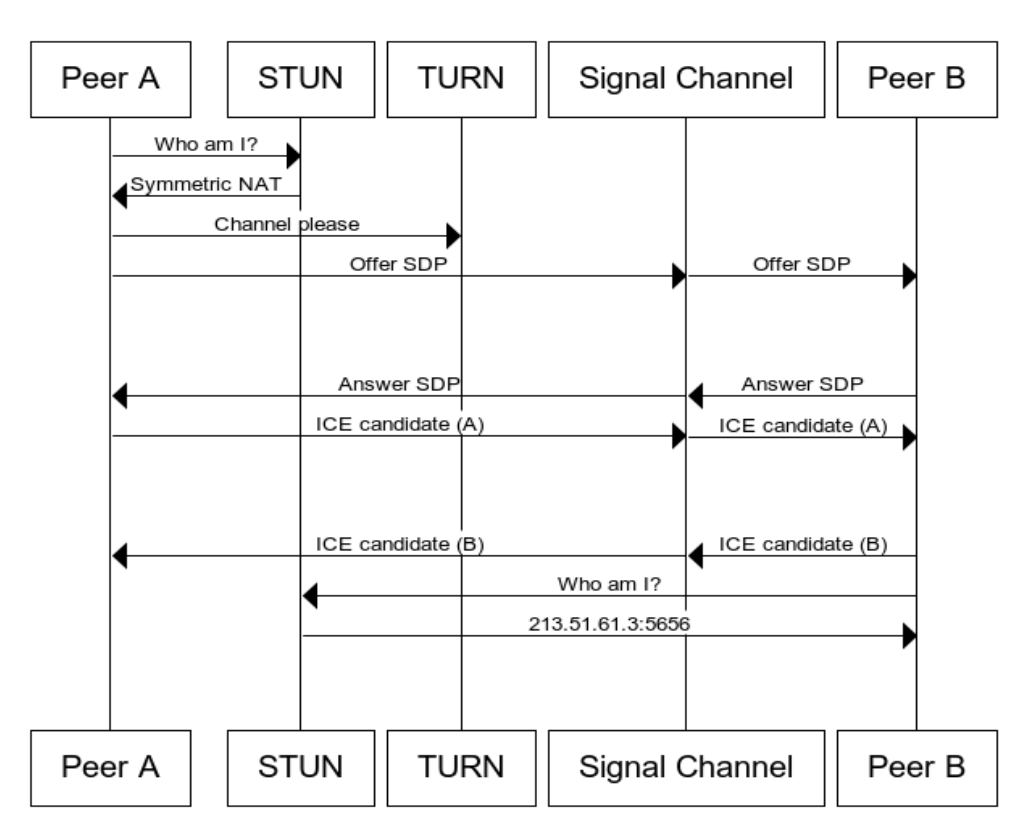
\includegraphics[width=10cm]{webRTC.png}
\end{center}
\caption{Call Service: webRTC Signalling Plane}
\label{fig:webrtc}
\end{figure}

\subsection{Codecs}

Before sending the media over a peer connection, it has to be compressed. 
Raw audio and video is simply too large to send efficiently in our current Internet infrastructure.
Likewise, after receiving media over a peer connection, it has to be decompressed. 
For this, use a media codec.

WebRTC has mandated three audio codecs and two video codecs:

\begin{enumerate}
    \item Audio - PCMU (G.711$\mu$) running at 8,000Hz with a single channel (mono).
    \item Audio - PCMA (G.711a) running at 8,000Hz with a single channel (mono).
    \item Audio - Opus running at 48,000Hz with two channels (stereo).
    \item Video - VP8.
    \item Video - H.264/AVC using Constrained Baseline Profile Level 1.2.
\end{enumerate} 

The technology is available on all modern browsers as well as on native clients for
all major platforms. The technologies behind WebRTC are implemented as an open web 
standard and available as regular JavaScript APIs in all major browsers. For native clients, 
like Android and iOS applications, a library is available that provides the same 
functionality.~\cite{UltimateGuideWebRTC}


\section{MATRIX}

Matrix is an open protocol for decentralised communication. It aims to make 
communication platforms interoperable and federated.

The main idea is to make real-time communication work seamlessly between different chat 
service providers, allowing users with accounts at one communications service provider to 
easily communicate with users of a different service provider.

Users have the privilege to communicate with people outside the Matrix network through bridges, 
which connect previously established communication networks, such as Slack and IRC, to the Matrix network.
With bridges, you do not have to use different apps to talk to different people. Whatever Matrix 
client you choose, you can talk to anyone inside or outside the Matrix network.

Matrix gives users total control over their communication by letting them run or select their own 
server while still participating in a global network, rather than being locked in silos 
like Signal, WhatsApp, Telegram, Slack etc. 

The key feature of Matrix is that no single server hosts or controls a given conversation - instead, 
as one user communicates with another, the conversation gets replicated equally across the servers - meaning 
all the participants equally share ownership over the conversation and its history. 
There is never a central point of control or authority, 
unless everyone decides to use the same server.~\cite{MATRIXorgOpenProtocol}

By default, Matrix uses simple HTTPS+JSON APIs as its baseline transport, but also embraces 
more sophisticated transports such as WebSockets or ultra-low bandwidth Matric via CoAP+Noise.~\cite{MATRIX}

Applications using the Matrix protocol, called Matrix clients, have all the features one would
want and expect from a modern chat app: instant messaging, group chats, audio and video calls, 
searchable message history, synchronization across all devices, as well as end to end encryption.
Element is the best known Matrix client.
Via Matrix, Element is able to bridge communications like IRC, Slack and Telegram into the app.~\cite{RumaMATRIX}

\begin{figure}[h]
    \begin{center}
        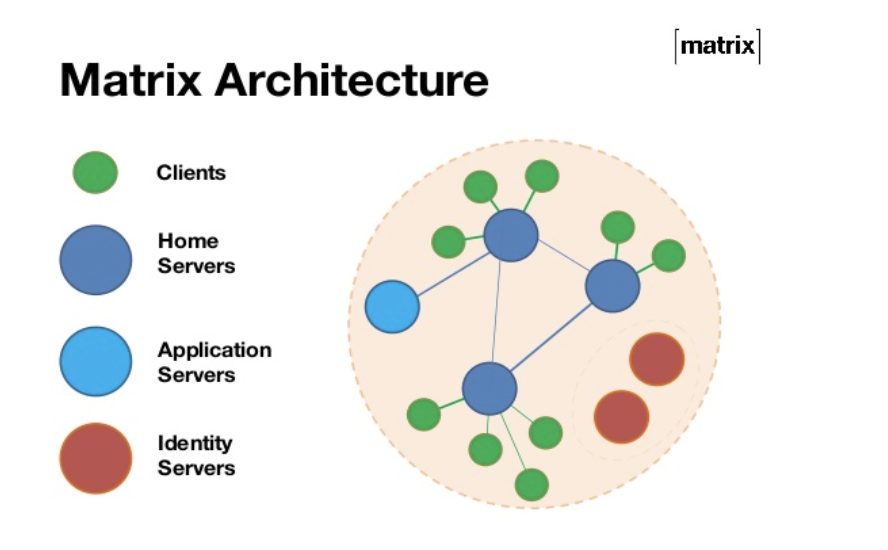
\includegraphics[width=10cm]{matrix.png}
    \end{center}
    \caption{An example of a Matrix Architecture, illustrated very simply using abstract coloring.}
    \label{fig:matrix}
\end{figure}

\subsection{Why MATRIX?}

As a result of several chat services not being interoperable with each other, people are 
forced to use multiple services to communicate.
However, since Matrix is federated, just like email, you can freely communicate across a 
global network, without having to use specific services based on which ones your friends, 
family, and colleagues use.

Another major problem with online communication today is that most of the services you
use are operated by commercial organizations, forcing you to trust them to manage your data.
But because Matrix is federated, you have control over where your data is stored and who has access to it.~\cite{RumaWhyMatrix}
\section{REST API}

A REST API is an application programming interface that conforms to the constraints of the REST 
architectural style and allows for interaction with RESTful web services.

REST is not a standard, but rather a set of recommendations and constraints for 
RESTful web services. These include:

\begin{enumerate}
    \item \textbf{Client-Server.} System ‘A’ makes an HTTP request to a URL hosted by 
    System ‘B’, which returns a response.
    It is identical to how a browser works: The application first requests a specific URL, the request is then routed to a web server that returns an HTML page. 
    This page may contain references to images, style sheets, and JavaScript, 
    which incur further requests and responses.

    \item \textbf{Stateless.} REST is stateless: the client request should contain all the information necessary to respond to a request. In other words, it should be possible to
    make two or more HTTP requests in any order and the same responses will be received.

    \item \textbf{Cacheable.} A response should be defined as cacheable or not.
    
    \item \textbf{Layered.} The requesting client need not know whether it’s communicating 
    with the actual server, a proxy, or any other intermediary.~\cite{DevelopersRestAPI}
\end{enumerate}

The working first involves sending a request from the client to the server in the form of web URLs, 
using the HTTP GET, POST, PUT or DELETE methods. After that, a response is retrieved from the server 
in the form of a resource which can be anything like HTML, XML, Image, or JSON.~\cite{WhatisRESTAPI}

\begin{figure}
    \begin{center}
        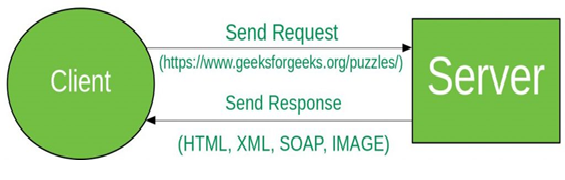
\includegraphics[width=8cm]{restapi.png}
    \end{center}
    \caption{A simple illustration of a REST API request-response.}
    \label{fig:restapi}
\end{figure}

In HTTP five methods are commonly used in a REST-based Architecture i.e. POST, GET, PUT, PATCH, and DELETE. These methods correspond to create, read, 
update, and delete (or CRUD) operations respectively.~\cite{GeeksRestAPI}

\section{GraphQL}

GraphQL is a query language and server-side runtime for Application Programming Interfaces (APIs) 
that prioritizes giving clients exactly the data they request and nothing more. 
GraphQL is designed to make APIs fast, flexible, and developer-friendly. It is not tied 
to any specific database or storage engine and is instead backed by existing code and data.

API developers use GraphQL to create a schema to describe all the possible data that clients can query through that service. This schema is made up of object types, which define which kind of object can be
requested and what fields it has. As queries come in, GraphQL validates the queries against the schema. 
GraphQL then executes the validated queries.

The API developer attaches each field in a schema to a function called a resolver. 
During execution, the resolver is called to produce the value.~\cite{WhatisGraphQL}

GraphQL follows the same set of constraints as REST APIs, but it organizes data into a 
graph using one interface. Objects are represented by nodes (defined using the GraphQL schema), 
and the relationship between nodes is represented by edges in the graph. Each object is then backed by a resolver that accesses the server’s data.

When a GraphQL server responds to an end user’s request, it begins with the query root,
and the resolver executes every field on the requested object. A key-value map houses each field’s
values, and some return another object selecting another set of fields. This continues until only a 
string or a number is returned. The server then responds with a nested set of objects, as requested by the end-user.~\cite{RubrikGraphQL}

\begin{figure}
    \begin{center}
        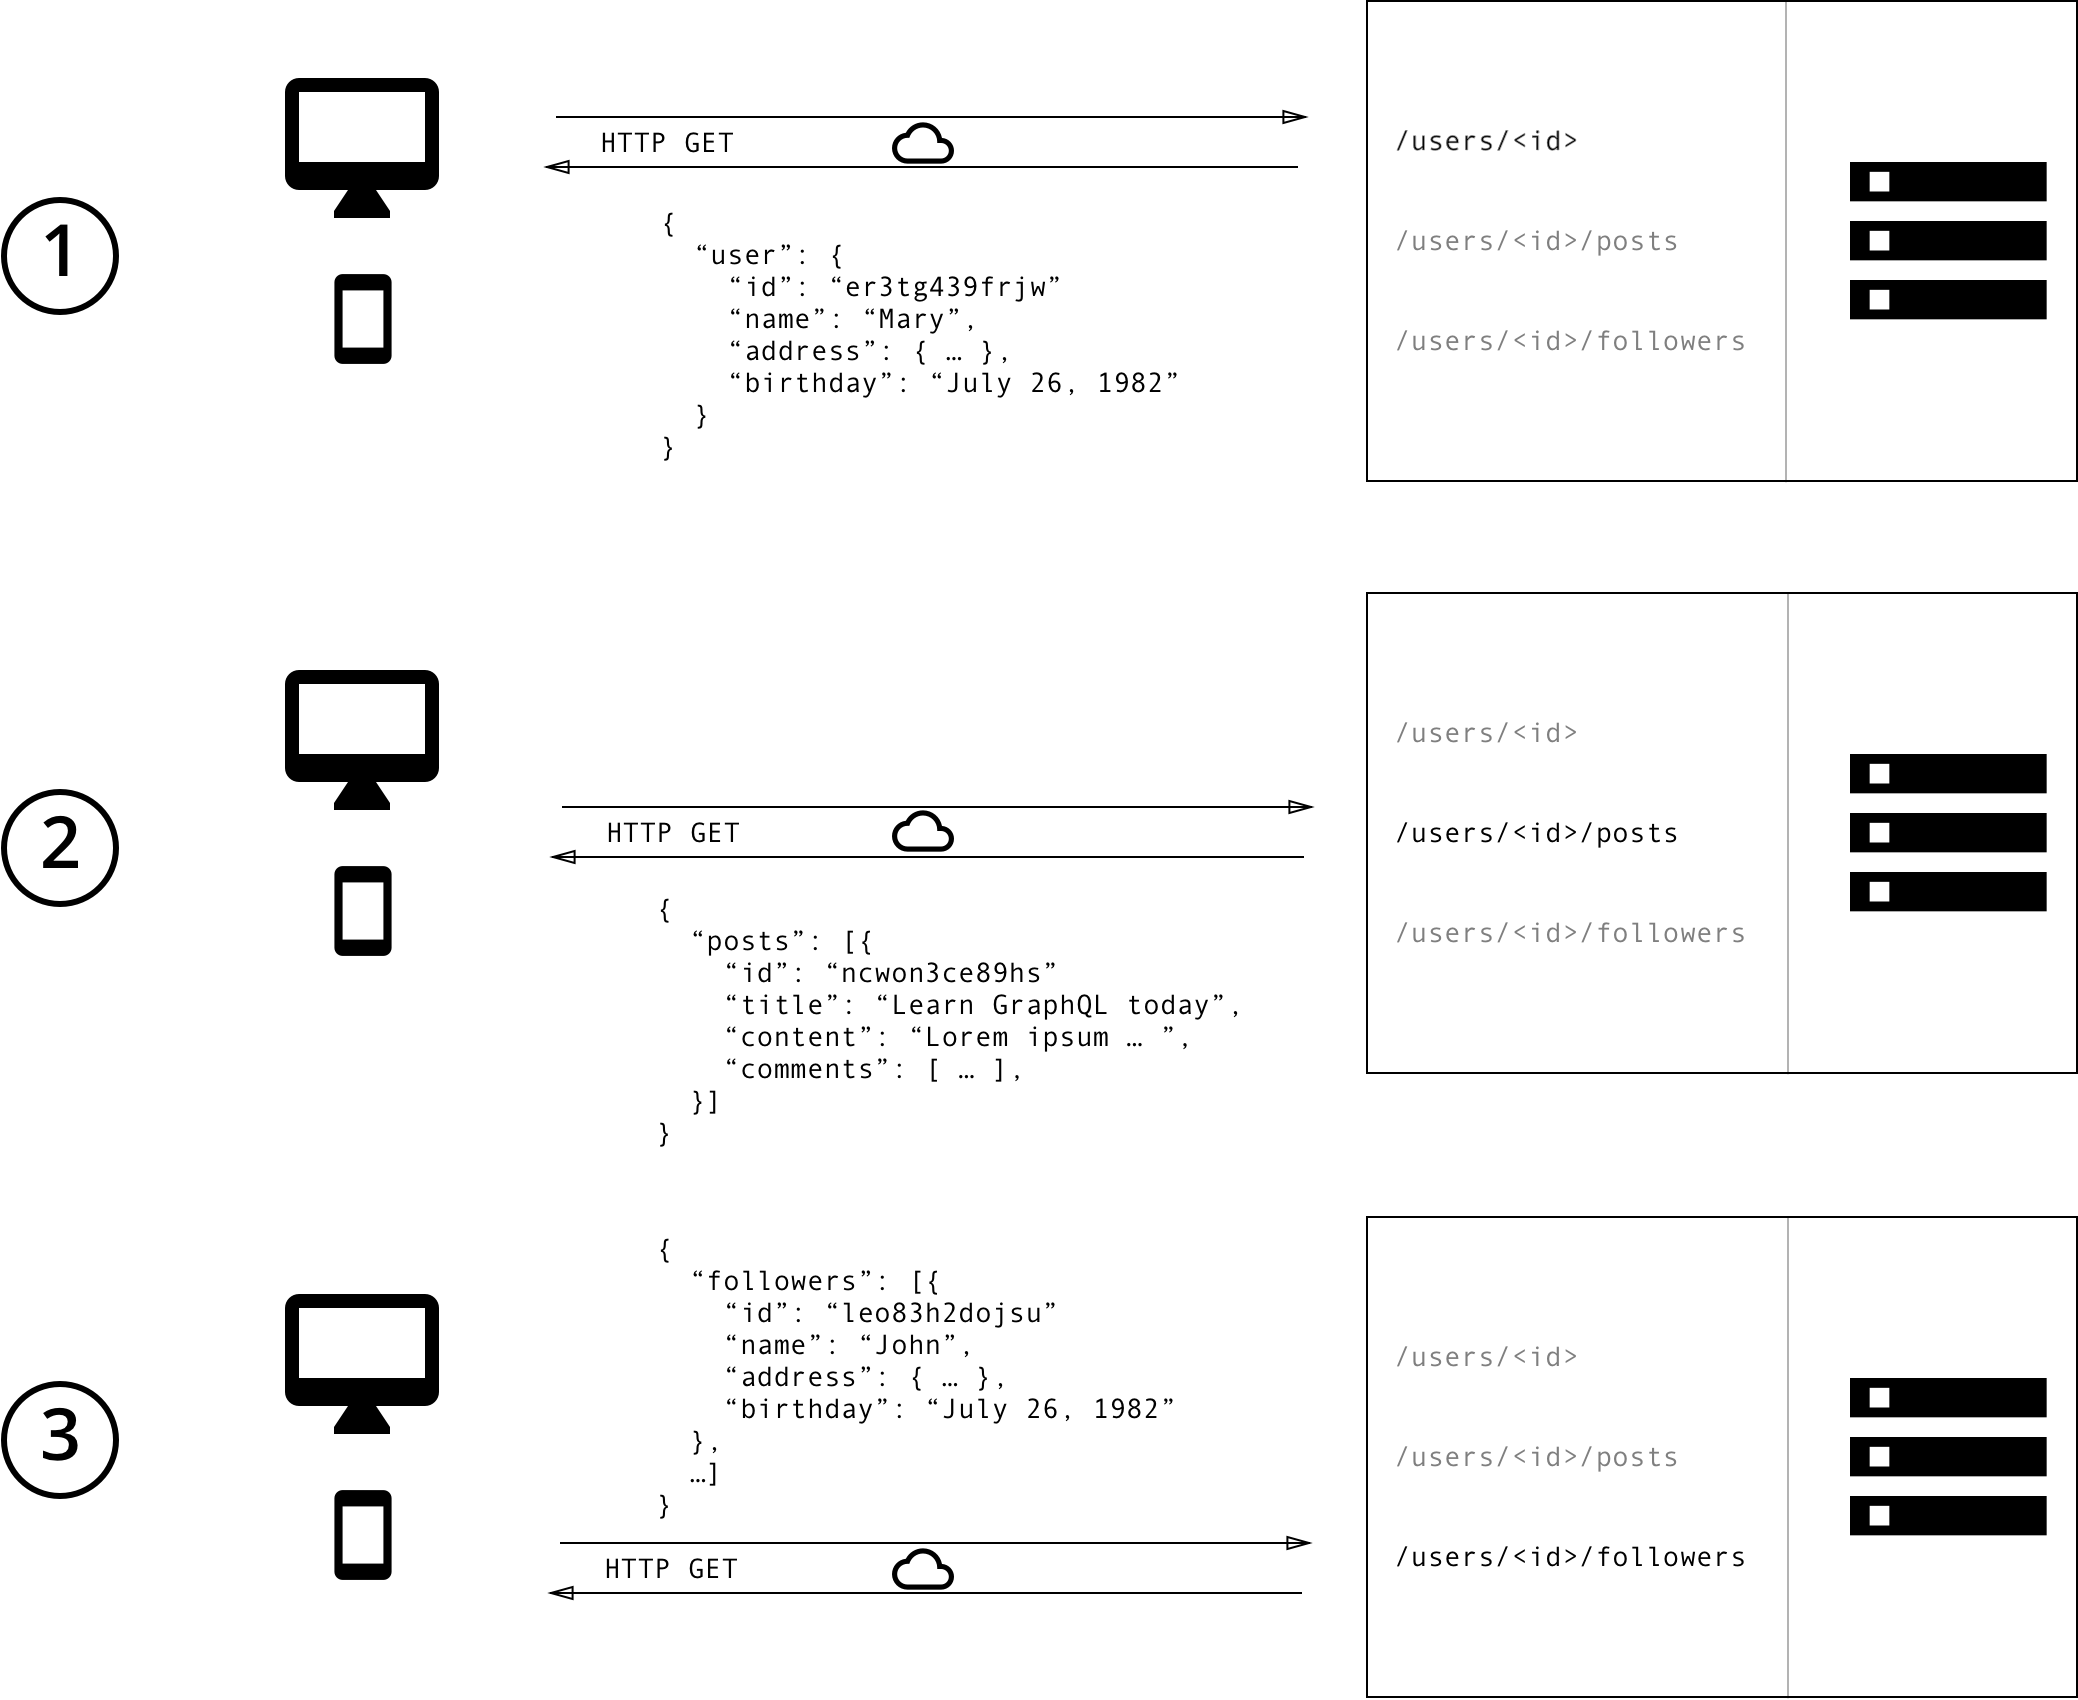
\includegraphics[width=15cm]{graphql-rest.png}
    \end{center}
    \caption{GraphQL can handle the tasks of multiple REST endpoints, 
    neither overfetching, nor underfetching,
    offering the exact data format as requested by the client.}
    \label{fig:graphql}
\end{figure}
  
\subsection{How does GraphQL excel REST API?}

\subsubsection{Data Fetching}

With a REST API, data would be gathered by accessing multiple endpoints. The application would  
end up having to make multiple requests to different endpoints to fetch the required data, and could lead to over fetching of data.
In GraphQL on the other hand, a single query to the GraphQL server that includes the concrete data requirements would be sufficient. The server would then respond with a JSON object where these requirements are fulfilled. Therefore using GraphQL, the client can specify exactly the data it needs in a query.

\subsubsection{Over-fetching and Under-fetching of Data}

One of the most common problems with REST is that of over-fetching and under-fetching. This happens because the only way for a client to download data is by hitting multiple endpoints that return fixed data structures.
GraphQL gives the clients the exact data they request for.

\subsubsection{Benefits of a Schema and Type System}

GraphQL uses a strong type system to define the capabilities of an API. All the types that are exposed in an API 
are written down in a schema using the GraphQL Schema Definition Language (SDL). This schema serves as the contract between the client and the server to define how a client can access the data.
Once the schema is defined, the teams working on frontend and backend can do their work without regular communication 
since they both are aware of the definite structure of the data that’s sent over the network.
Frontend teams can easily test their applications by mocking the required data structures. Once the server is ready, 
the switch can be flipped for the client apps to load the data from the actual API.

\subsubsection{Rapid Product Iterations on the Front-end}

A common pattern with REST APIs is to structure the endpoints according to the views inside the app for the client to get all required information for a particular view by simply accessing the corresponding endpoint. However, the major drawback of this approach is that it doesn’t allow for rapid iterations on the front end. 
With every change that is made to the UI, there is a high risk that now there is more or fewer data required than before.
Consequently, the backend needs to be adjusted as well to account for the new data needs. This notably slows down the ability to incorporate user feedback into a product. But owing to the flexible nature of GraphQL, changes on the client-side can be made without any extra work on the server. Since clients can specify their exact data requirements, 
no backend adjustments are required when the design and data need on the frontend change.

\subsubsection{Insightful Analytics on the Back-end}

GraphQL allows having fine-grained insights about the data that’s requested on the backend. As each client specifies exactly what information it’s interested in, it is possible to gain a deep understanding of how the available data is being used. This can for example help in evolving an API and deprecating specific fields that are not requested by any clients anymore.
With GraphQL, the developer can also do low-level performance monitoring of the requests that are processed by the server. 
GraphQL uses the concept of resolver functions to collect the data that’s requested by a client. Instrumenting and measuring 
performance of these resolvers provides crucial insights about bottlenecks in the system.~\cite{GraphQLvsREST}

\section{Neural Discrete Representation Learning}

Recent advances in generative modeling of images, audio, and videos have yielded impressive
samples and applications. At the same time, the challenges that follow these tasks are few-shot
learning, domain adaptation, or reinforcement learning heavily rely on learned representations from raw data.

Learning representations with continuous features have been used in much previous work but discrete representations are a potentially more natural fit for many applications. 
Discrete representations are a natural fit for complex reasoning, planning, and predictive learning
(e.g., if it rains, I will use an umbrella).

This concept of discrete representation gave rise to the Vector Quantization-Variational Autoencoder. 
This model relies on Vector Quantization with the combination of Variational Autoencoder framework with 
discrete latent representations through a novel parameterization of the posterior distribution of (discrete) 
latent given an observation.~\cite{oord2018neural}

\subsection{Vector Quantization - Variational Autoencoder (VQ-VAE)}

VAEs consist of the following parts: an encoder network which parameterised a posterior  
distribution $q(z|x)$ of discrete latent random variables $z$ given the input data $x$, a prior
distribution $p(z)$, and a decoder with a distribution $p(x|z)$ over input data.

Typically, the posteriors and priors in VAEs are assumed normally distributed with diagonal covariance. Extensions include autoregressive prior and posterior models, normalizing flows, 
and inverse autoregressive posteriors. VQ-VAE uses discrete latent variables which is a new way of training, by using vector quantization (VQ). The posterior and prior distributions are categorical, and the samples were drawn from these distributions index an embedding table. These embeddings
are then used as input into the decoder network.

\subsection{Discrete Latent Variables}

Let's define a latent embedding space $e \in R^{K \times D}$ where $K$ is the size of the discrete latent space 
(i.e., a $K$-way categorical), and $D$ is the dimensionality of each latent embedding vector $e_{i}$.
Note that there are $K$ embedding vectors $e_{i} \in R ^D$, $i\in{1, 2, ..., K}$.

The discrete latent variables $z$ are then calculated by a nearest 
neighbour look-up using the shared embedding space $e$ as shown in equation \ref{eqn:discrete}.

\begin{equation}
q(z = k|x) =
\begin{cases}
    1 & \text{for } k = \text{argmin}_{j} \| z_{e}(x) - e_{j} \|_{2} \\
    0 & \text{otherwise}
\end{cases}
\label{eqn:discrete}
\end{equation} 

where $z _e(x)$ is the output of the encoder network.

The input to the decoder is the corresponding embedding vector $e _k$ as given in equation \ref{eqn:decoder}
\begin{equation}
    z _q(x) = e _k, \text{where } k= \text{argmin} _j \| z _e(x) - e _j \| _2
    \label{eqn:decoder}
\end{equation}

\subsection{Learning}

\begin{figure}[h]
    \begin{center}
        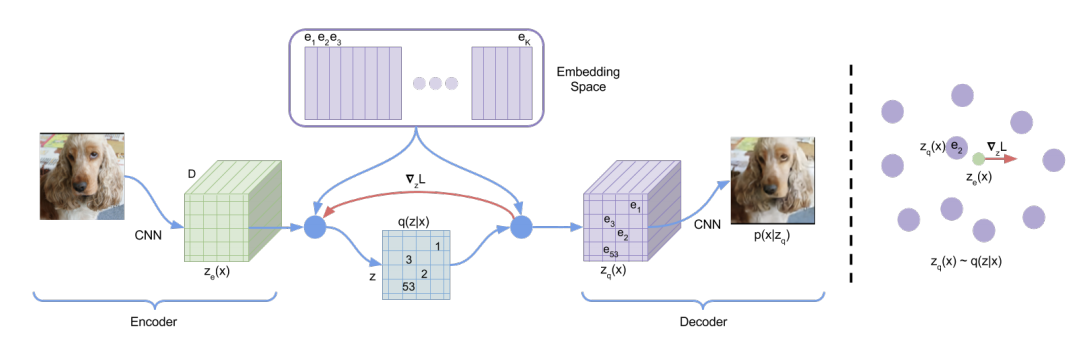
\includegraphics[width=15cm]{vqvae.png}
    \end{center}
    \caption{Left: A figure describing the VQ-VAE. Right: Visualisation of the embedding space. The
    output of the encoder $z(x)$ is mapped to the nearest point $e _2$. The gradient $\nabla _z L$ (in red) will push the
    encoder to change its output, which could alter the configuration in the next forward pass.}
    \label{fig:vqvae}
\end{figure}

During forwarding computation, the nearest embedding $z _q(x)$ is passed to the decoder,
and during the backward pass, the gradient $\nabla _z L$ is passed unaltered to the encoder. 
Since the output representation of the encoder and the input to the decoder share the same $D$
dimensional space, the gradients contain useful information for how the encoder has to change its 
output to lower the reconstruction loss.

As seen in figure \ref{fig:vqvae} (right), the gradient can push the encoder’s output to be discretized 
differently in the next forward pass, because the assignment in equation \ref{eqn:discrete} will be different

The log-likelihood of the complete model $\log p(x)$ can be evaluated as follows:

\begin{equation}
    \log p(x) = \log \sum _k p(x|z _k) p(z _k)
    \label{eqn:modellog}
\end{equation}

Because the decoder $p(x|z)$ is trained with $z = z _q(x)$ from MAP-inference, the decoder
should not allocate any probability mass to $p(x|z)$ for $z \neq z _q(x)$ once it has fully converged.

Thus, the authors concluded.~\cite{razavi2019generating, oord2018neural}
\begin{equation}
    \log p(x) \approx \log p(x|z _q(x))p(z _q(x))
\end{equation}

\subsection{Prior}

The author also stated a prior distribution can be made autoregressive by depending on $z$ 
in the feature map as it is a categorical distribution over the discrete latent $p(z)$. 
While training the VQ-VAE the prior is kept constant and uniform. After training, fit an autoregressive distribution over $z$, $p(z)$, so that it can generate $x$ via ancestral sampling.

% Add FOMM (MonkeyNet).
\section{Distilling the Knowledge in a Neural Network}

An ensemble of models is a simple method of improving the performance of a machine learning algorithm.
It works by training many different models on the same data and then considering the average of their predictions.
However, an ensemble of models is difficult to incorporate into most end-user devices, because all models belonging to the ensemble need to operate to arrive at a useful prediction.

Rich Caruana et al.~\cite{caruana2015compression} have shown it is possible to compress the knowledge
represented by an ensemble of models into a single model with much fewer parameters. This process, called
Knowledge Distillation allows the creation of 'specialist' models which are much easier to deploy widely.

The reason an ensemble of models generalizes so well on large datasets is that the average results of the entire ensemble are considered. The dataset could contain noise and outliers, but an ensemble manages to avoid overfitting because of taking the average of all the model outputs. We cannot expect a smaller model to generalize to large 
datasets without heavy feature engineering, removing many features from the dataset to help the smaller model cope.

The process of knowledge distillation requires us to find 'soft targets'. A soft target is a prediction made by the ensemble of models for an input. Unlike hard targets (i.e. targets that are difficult to make sense of), 
soft targets need to have high entropy and low variance to provide much more information per training case.

\begin{figure}[h]
    \begin{center}
        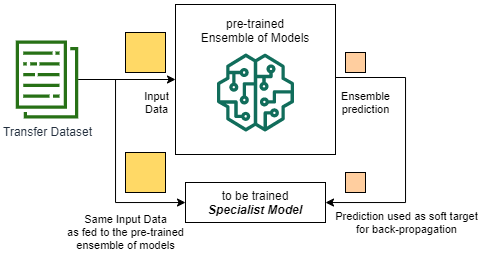
\includegraphics[width=10cm]{KnowledgeDistillation.png}
    \end{center}
    \caption{An illustration of the process of training a specialist model using Knowledge Distillation.
    The specialist models can thus be trained fast, and in parallel.}
    \label{fig:distillation}
\end{figure}

As can be seen in figure~\ref{fig:distillation}, we feed the same training/transfer input 
from the transfer dataset into both the specialist model and the ensemble of models. 
The output of the ensemble of models is then used as a soft target to the specialist model.
The specialist model can thus be trained rapidly, and multiple specialist models can also 
be trained and tested in parallel, and on much higher learning rates, unlike a Mixture of Experts, 
where multiple models are learning only a specific part of the dataset, assigned to the models 
based on a gating network mechanism.

\subsection{Discussion}

Geoffrey Hinton et al.~\cite{hinton2015distilling} were able to train a large, highly regularized
ensemble of models on various tasks, including the MNIST handwritten digit dataset and Speech 
Recognition of deep acoustic models similar to the one used by Android voice search. Nearly all of the improvement achieved by training an ensemble of deep neural nets could be trained into a single specialist
model of the same size, achieving similar results, and being easier to deploy to end-user devices.

From these findings, we can thus attempt training smaller specialist models using existing pre-trained models.
These smaller models can thus be deployed widely.
\section{Efficient text-search using TF-IDF}

TF-IDF stands for Term Frequency-Inverse Document Frequency. 
The TF-IDF weight is a weight often used in information 
retrieval and text mining. Variations of the TF-IDF weighting 
scheme are often used by search engines in scoring and ranking 
a document’s relevance given a query. 
This weight is a statistical measure used to evaluate how 
important a word is to a document in a collection or corpus. 
The importance increases proportionally to the number of times 
a word appears in the document but is offset by the frequency 
of the word in the corpus.

TF-IDF is a weighting scheme that assigns each term in a 
document a weight based on its Term Frequency (TF) and 
Inverse Document Frequency (IDF). The terms with higher 
weight scores are considered to be more important.

Typically, the TF-IDF weight is composed by two terms:
\begin{enumerate}
    \item Normalized Term Frequency (TF)
    \item Inverse Document Frequency (IDF)
\end{enumerate}

Therefore, Term Frequency is a measure of how frequently a 
term occurs in a document.
\begin{equation}
    tf(t, D) = \frac{\text{Number of times the term } t \text{ appears in document } D}{\text{Total number of terms in the document}}
    \label{eqn:tf}
\end{equation}

Inverse Document Frequency is a measure of how important a term is.~\cite{tfidftutorial}
\begin{equation}
    idf(t, D) = \log \frac{N}{n _t}
    \label{eqn:idf}
\end{equation}
where, $N =$ Total number of documents, $n _t =$ Number of documents having the term $t$ in it.

We now combine both to produce a composite weight for each term in each document.
\begin{equation}
    tfidf(t,D) = tf(t,D) \times idf(t,D)
    \label{eqn:tfidf}
\end{equation}
Also, The TF-IDF score/relevancy for a multi-term query $q = (t 1 , . . . , t_m)$ is~\cite{tfidfFormulae}:
\begin{equation}
    score _{tfidf}(q, d, D) = \sum^{m}_{i = 1} score _{tfidf}(t _i, d, D)
    \label{eqn:score}
\end{equation}

\subsubsection{Use of TF-IDF text search in an example}

Suppose our search engine contained the following three documents,

\textbf{Document A:} "the mouse played with the cat"

\textbf{Document B:} "the quick brown fox jumped over the lazy dog"

\textbf{Document C:} "dog 1 and dog 2 ate the hot dog"

We compute the TF-IDF vector for each document like so~\cite{tfidfExample}:

\textbf{Document A:} "the mouse played with the cat"
\begin{figure}[h!]
    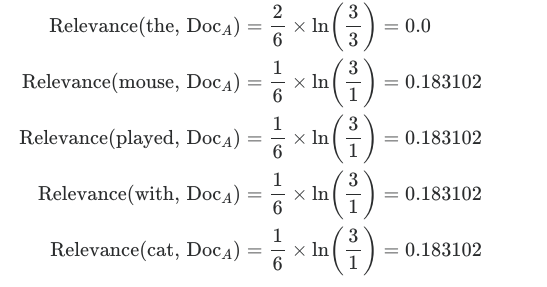
\includegraphics[width=8cm]{tfidf-example.png}
\end{figure}

\subsection{Compare query against a document}
\begin{enumerate}
    \item Find the TF-IDF vector for the document. This should be an easy, $O(1)$ lookup since we already computed the TF-IDF vector.
    \item Compute the TF-IDF vector for the query. (Note: technically, we are treating the query as if it were a new document. However, you should not recompute the IDF values: just use the ones you computed earlier.)
    \item Compute the cosine similarity between the document vector and the query vector.
    \item We can do this by comparing the TF-IDF vector for your query against all the document TF-IDF vectors and compute how similar your query vector is to each document by exploiting properties of the cosine function and the dot product.
\end{enumerate}

We determine the $K$ documents of the collection with the highest vector space 
scores on the query $q$. Typically, we seek these $K$ top documents ordered by 
score in decreasing order; for instance many search engines use $K = 10$ to retrieve 
and rank-order the first page of the ten best results.~\cite{tfidfExample}

\subsubsection{Time Complexity}

The time complexity of this algorithm is:
\begin{equation}
    O(|Q| |D| |T|) = O(|D| |T|)
\end{equation}

we consider $|Q|$ fixed, where $Q$ is the set of words in the query and $D$ is the set of all documents.

Also, if the $D$ is the set of only the matching documents, then
since scores is a priority queue (at least in doc-at-time-scheme) built on heap, 
putting every $d$ into takes $\log K$. Therefore we can estimate it as $O(|D| \log K )$.


\section{Comparison between Key Technologies}

This section introduces key technologies, software packages and tools.
It is important to note that NVIDIA Maxine will not be used while building this project.
The subsection dedicated to NVIDIA Maxine contains a key observation which 
could possibly affect the project, hence it was added.

\subsection{NVIDIA Maxine}

NVIDIA Maxine is a fully accelerated platform SDK for developers of video 
conferencing services to build and deploy AI-powered features that use state-of-the-art 
models in their cloud. Video conferencing applications based on Maxine can reduce video bandwidth usage down to one-tenth of H.264 using AI video compression, dramatically reducing costs.

Maxine includes APIs for the latest innovations from NVIDIA research such as face alignment, 
gaze correction, face re-lighting, and real-time translation in addition to capabilities such as super-resolution, noise removal, closed captioning, and virtual assistants. These capabilities are fully accelerated on NVIDIA GPUs to run in real-time video streaming applications in the cloud.

Maxine-based applications let service providers offer the same features to every user on any device,
including computers, tablets, and phones. Applications built with Maxine can easily be deployed as 
microservices that scale to hundreds of thousands of streams in a Kubernetes environment.~\cite{Maxine}

\subsubsection{Features}

\begin{itemize}
    \item \textbf{Easy to use SDK}: Includes libraries, tools and example pipelines 
    for developers to quickly add AI features to their applications.
    \item \textbf{Ultra-low Bandwidth}: AI Video Compression uses one-tenth the 
    bandwidth of H.264 video compression standard.
    \item \textbf{State-of-the-art AI model}: Includes pre-trained models with thousands of hours 
    of training on NVIDIA DGX\texttrademark A100.
    \item \textbf{Fully GPU Accelerated}: Optimizes end-to-end pipelines for the highest performance 
    on NVIDIA Tensor Cores GPUs.
\end{itemize}

\subsubsection{Key Technologies}

\begin{itemize}
    \item \textbf{Reduce Video Bandwidth compared to H.264}: 
    With AI-based video compression technology running on \textbf{NVIDIA GPUs}, 
    developers can reduce bandwidth use down to one-tenth of the bandwidth needed 
    for the H.264 video compression standard. This cuts costs for providers and 
    delivers a smoother video conferencing experience for end-users, who can enjoy 
    more AI-powered services while streaming less data on their computers, tablets, and phones.
    
    \item \textbf{Face Re-Animation}:
    Using new AI research, the key facial points of each person on a video call can be identified
    and then used to reanimate a person’s face on the other side using a still image
    of the call with Generative Adversarial Networks (GANs).
    
    These key points can be used for face alignment, where faces are rotated so that
    people appear to be facing each other during a call, as well as gaze correction 
    to help simulate eye contact, even if a person’s camera isn’t aligned with their screen.
    
    Developers can also add features that allow call participants to choose their
    own avatars that are realistically animated in real-time by their voice and emotional tone.

    \item \textbf{Video and Audio Effects}:
    AI-based super-resolution and artifact reduction can convert lower resolutions to higher
    resolution videos in real-time which help to lower the bandwidth requirements for video 
    conference providers, as well as improve the call experience for users with lower bandwidth. 
    Developers can add features to filter out common background noise and frame the camera on a user’s 
    face for a more personal and engaging conversation.
    
    Additional AI models can help remove noise from low-light conditions creating a more appealing picture.

    \item \textbf{Conversational AI}:
    Maxine-based applications can use NVIDIA Jarvis, a fully accelerated conversational
    AI framework with state-of-the-art models optimized for real-time performance. Using Jarvis, 
    developers can integrate virtual assistants to take notes, set action items, and answer questions in human-like voices.
    
    Additional conversational AI services such as translations, closed captioning and transcriptions help ensure everyone can understand what’s being discussed on the call.
\end{itemize}

\subsubsection{Observation}

NVIDIA Maxine needs all of its devices to have NVIDIA hardware or access to the NVIDIA cloud. 
This reduces the customer base because of its cost and the huge unavailability of GPUs.

It is therefore important to understand that dependence on compute-intensive hardware could
currently, be the only barrier to building effective applications using Neural Networks.

\subsection{Comfort Noise}

Comfort noise is an audibly soft, synthetic background noise that was introduced in wireless communications 
mainly to overcome the issues of artificial silence which occurs in voice activity detection systems.
The issues of receiving prolonged periods of artificial silence would include:

\begin{itemize}
    \item The listener disconnecting prematurely believing transmission has been lost.
    \item The speech does not sound smooth, since the voice activity detector would abruptly cut the signal as an attempt to save bandwidth, but this would give the listener a perception that the voice quality has worsened.
    \item The sudden changes in voice amplitude, punctuated by repeated gaps of silence would be jarring to the listener.
\end{itemize}

As can be observed, the above issues are not technical. Engineers arrived at a simple solution that involved adding comfort noise to the communication. This noise is added at the receiving end of the communication, and not transmitted.~\cite{ComfortNoise}
Such a setup helps save bandwidth while also circumventing the issues described above.
\section{PeerJS}

The PeerJS library is aimed to simplify the peer-to-peer connection management. 
PeerJS wraps the browser's WebRTC implementation to provide a complete, configurable, 
and easy-to-use peer-to-peer connection API. 
With PeerJS, peers are identified by simply using an ID, a string that the peer 
can choose itself, or have a server generate one. 
Equipped with an ID, a peer can create a P2P data or media stream connection to a remote peer.~\cite{PeerJSsimplifiesWebRTC}

\subsection{PeerJS Server}

Although WebRTC promises peer-to-peer communication, a server is still required to 
act as a connection broker, and handle signalling.

PeerJS provides an open source implementation of this connection broker 
server named PeerJS Server, written in Node.js.Users can run their own Server, 
or are at leisure to opt for the cloud-hosted version of PeerServer provided for free.
To broker connections, PeerJS connects to a PeerServer. The PeerJS Server acts ONLY as 
a connection broker, and it has to be noted that no peer-to-peer data goes through the server.~\cite{TamingWebRTCwithPeerJS}

To make the P2P connection work seamlessly, we will build the neural network encoder and 
integrate it into WebRTC possibly using the P2P library.

\section{CouchDB for Offline first design}

\subsection{What is RxDB?}

RxDB (Reactive Database) is a NoSQL database for JavaScript Applications 
like websites, hybrid Apps, Electron-Apps, Progressive Web Apps and NodeJs.

RxDb allows you to not only query the current state but subscribe to all state changes.
Therefore it is useful in UI-based real time applications and makes it easy to develop 
and adds great performance benefits.
RxDB provides modules for realtime replication with any CouchDB compliant endpoint and 
also with custom GraphQL endpoints to replicate data between your clients and server.~\cite{RxDB}

\subsection{What is PouchDB?}

PouchDB is an open-source JavaScript database inspired by Apache CouchDB which 
runs well within the browser. PouchDB helps build applications that work as well 
offline as they do online. It allows applications to store data locally while offline, 
then synchronize it with CouchDB and compatible servers when the application is back 
online, keeping the user's data in sync no matter where they next login.~\cite{PouchGuide}

\subsection{What is CouchDB?}

CouchDB is (categorised as) a NoSQL database.A CouchDB database does not have a schema, 
or pre-defined data structures such as tables. Data is stored as JSON document. 
The structure of the data, or document, can change dynamically to accommodate evolving needs.  
CouchDB is a peer based distributed database system. Any number of CouchDB hosts 
(servers and offline-clients) can have independent "replica copies" of the same database, 
where applications have full database interactivity (query, add, edit, delete). 
When back online or on a schedule, database changes can be replicated bi-directionally.
It is schema-free.~\cite{CouchConfluence}

\subsection{Offline First Design}

\begin{figure}[h!]
    \begin{center}
        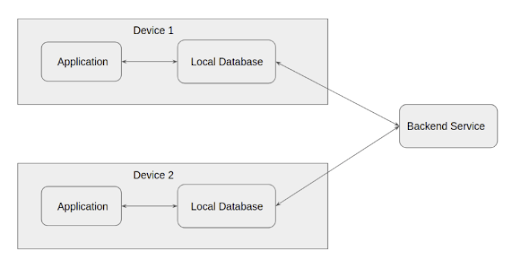
\includegraphics[width=10cm]{offline-first.png}
    \end{center}
    \caption{Simple architecture of the offline first model}
    \label{fig:offline-first}
\end{figure}

Offline first is an application development paradigm where developers ensure that the 
functionality of an app is unaffected by intermittent lack of a network connection. 
In addition offline first usually implies the ability to sync data between multiple devices
For an app to be offline first we need to make sure that both code and the data required 
for it to function are not dependent on the presence of the network.
Mobile applications do need to do something extra to make code available offline,
Web Applications however can include service workers to achieve the same.
With service workers we need to worry about when it is safe to update the code. 
Refer to figure \ref{fig:offline-first}.

A simple solution to making data available offline is to have a local database 
that you read and write to. The database can then be replicated to and from a 
server whenever a network is available.~\cite{HasuraOfflineFirst}


\subsection{Push-pull replication}

With RxDB you can do a two-way replication(push-pull replication) with a GraphQL endpoint. 
This allows you to replicate data from the server into the client-side database and then 
query and modify it in realtime.
When the user is offline, you still can use the data and later sync it with the server 
when the client is online again.

\textbf{Pros}
\begin{enumerate}
    \item GraphQL-replication is faster and needs less resources.
    \item You do not need a couchdb-compliant endpoint, only a graphql-endpoint.
\end{enumerate}

\textbf{Cons}
\begin{enumerate}
    \item You can not replicate multiple databases with each other.
    \item It is assumed that the graphql-server is the single source of truth.
    \item You have to set up things at the server side while with couchdb-sync 
    you only have to start a server.~\cite{RxDBreplication}
\end{enumerate}


\subsection{Conflict resolution}
If the app can be used from multiple devices, it is possible for the user to make 
conflicting changes on different devices.

\begin{itemize}
    \item Simplest way to handle conflicts is to assume that they don’t matter and 
    users will simply correct the data later. This approach is also known as last-write-wins.
\end{itemize}

Assuming we do want to detect and resolve conflicts, there are many broad approaches, 
one of them which pouchDB uses is:

\subsubsection{Version the objects:}

Every time a change is made a new version is created. In addition the parent version for a given 
version is also kept track. A conflict can be identified by the fact that two versions have the 
same parent. Two generic auto merge strategies are:

\begin{enumerate}
    \item \textbf{Last write wins}: Here we will simply take the last revision to 
    reach the server as the final value.
    \item \textbf{Merge by fields}: If the two devices modified different fields 
    of the object, it might be possible to auto merge by taking the new fields from both objects.
\end{enumerate}

In the above approach merging is done by the server and clients simply fetch the merged value. 
However if you need user intervention to resolve a conflict you need to do the merge on the client.
This will require all clients to store the version history of the document as well. A problem with this 
is that clients can independently merge the document creating new multiple merge revisions.
Clients need to handle this (For example by examining the history and ignoring one of the merge versions).

PouchDB and CouchDB handle this by using a hash of the document contents as the object version. So if two 
different devices resolve the conflict the exact same way they will end up with the exact same version id.

\subsubsection{How do we delete an object?}

A simple way to delete objects is to have a "deleted" flag in the object. 
Merge function can then decide what to do if a deleted object has been modified. 
On the client, any object with the deleted flag set can be immediately purged as 
there will be no more updates to it. On the server ideally we would want to know 
that all clients have deleted the object before purging the object. The not so ideal 
but practical alternative is to periodically purge old objects.

\subsubsection{Who uses this currently?}

PouchDB and CouchDB follow the above model. In this setup, versions are stored both on the client and 
the server. When there is a conflict a deterministic algorithm auto picks a winning version.~\cite{HasuraOfflineFirst}

\subsection{Eventual consistency via CAP theorem}

\begin{figure}[h!]
    \begin{center}
        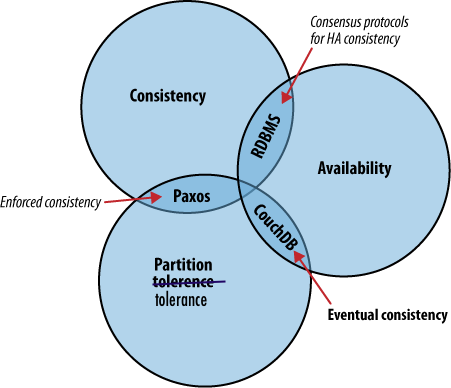
\includegraphics[width=10cm]{cap.png}
    \end{center}
    \caption{CAP Theorem. No database can offer the perfect solution for CAP.}
    \label{fig:cap}
\end{figure}

A distributed system is a system that operates robustly over a wide network. 
A particular feature of network computing is that network links can potentially 
disappear, and there are plenty of strategies for managing this type of network 
segmentation. CouchDB differs from others by accepting eventual consistency, 
as opposed to putting absolute consistency ahead of raw availability like 
RDBMS or Paxos. What these systems have in common is an awareness that data 
acts differently when many people are accessing it simultaneously. 
Their approaches differ when it comes to which aspects of consistency, 
availability, or partition tolerance they prioritize. Refer to figure \ref{fig:cap}.

The CAP theorem describes a few different strategies for distributing application 
logic across networks. CouchDB’s solution uses replication to propagate application 
changes across participating nodes. This is a fundamentally different approach from 
consensus algorithms and relational databases, which operate at different intersections 
of consistency, availability, and partition tolerance.

\begin{itemize}
    \item \textbf{Consistency}: All database clients see the same data, even with concurrent updates.
    \item \textbf{Availability}: All database clients are able to access some version of the data.
    \item \textbf{Partition tolerance}: The database can be split over multiple servers.
\end{itemize}

If availability is a priority, we can let clients write data to one node of the 
database without waiting for other nodes to come into agreement. If the database 
knows how to take care of reconciling these operations between nodes, we achieve 
a sort of “eventual consistency” in exchange for high availability.

\subsection{MapReduce algorithm}

CouchDB uses MapReduce to compute the results of a view. MapReduce makes use of two 
functions, “map” and “reduce,” which are applied to each document in isolation. 
Being able to isolate these operations means that view computation lends itself 
to parallel and incremental computation. More important, because these functions 
produce key/value pairs, CouchDB is able to insert them into the B-tree storage engine, 
sorted by key. Lookups by key, or key range, are extremely efficient operations with a 
B-tree, described in big O notation as $O(log N)$ and $O(log N + K)$, respectively.~\cite{CouchDB}

% Add existing storage alternatives.

%\begin{tabular}{c c c}
    
\end{tabular}